\documentclass{article}
\usepackage{122}

\usepackage{graphicx}
\usepackage[hidelinks,bookmarks=false]{hyperref}
\usepackage{attachfile}

\title{Биоинформатика \\ Домашнее задание №1}

% \usepackage{xcolor}
% \pagecolor{black}
% \color{white}

\begin{document}
  \maketitle

  \section{Бактерия \href{https://en.wikipedia.org/wiki/Clostridium_botulinum}{Clostridium botulinum}}
  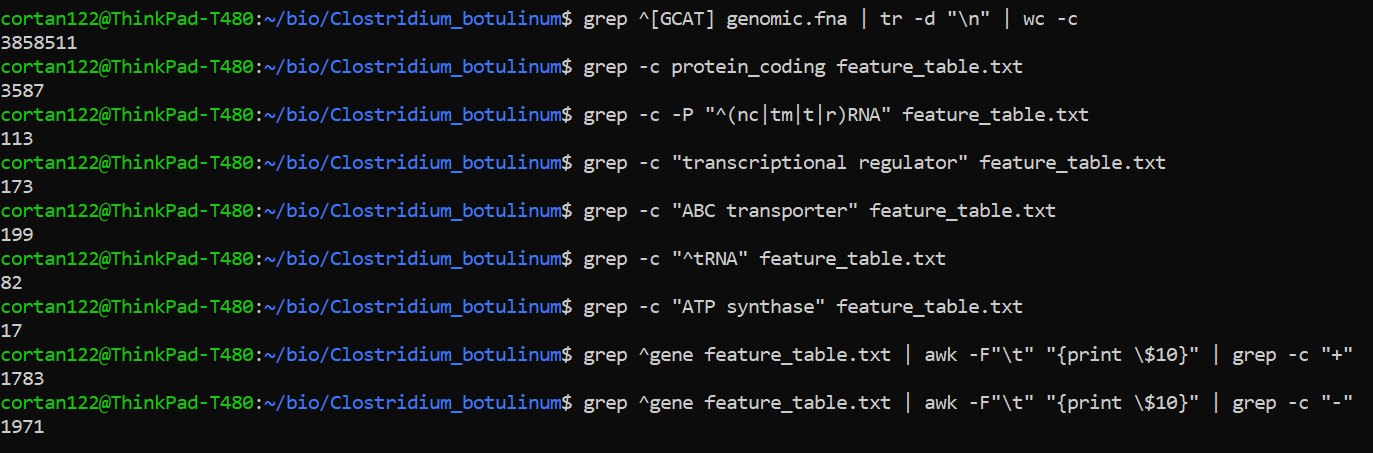
\includegraphics[width=\textwidth]{../bio/hw1/bacteria.png}

  \begin{enumerate}
    \item Какова длина генома (файл .fna) \\
      \textbf{Ответ:} $3858511$ bp
    \item Сколько генов, кодирующих белки? \\
      \textbf{Ответ:} $3587$
    \item Сколько рнк-генов? \\
      \textbf{Ответ:} $113$
    \item Сколько транскрипционных факторов? \\
      \textbf{Ответ:} $173$
    \item Сколько транспортных белков (ABC transporters)? \\
      \textbf{Ответ:} $199$
    \item Сколько tRNA? \\
      \textbf{Ответ:} $82$
    \item Сколько закодировано субъединиц АTP-synthase? \\
      \textbf{Ответ:} $17$
    \item Сколько генов закодировано на положительном, а сколько на отрицательном стренде? \\
      \textbf{Ответ:} $1783$ на положительном и $1971$ на отрицательном
  \end{enumerate}

  \section{Ген \href{https://en.wikipedia.org/wiki/SEP15}{SEP15} (или SELENOF)}
  \subsection{В геномном браузере \href{https://genome-euro.ucsc.edu/cgi-bin/hgTracks?db=hg38&position=chr1\%3A86862445\%2D86914365}{UCSC} отобразить все изоформы гена, а также SNPs (common and clinically relevant), участки консервативности среди позвоночных и транспозоны}
  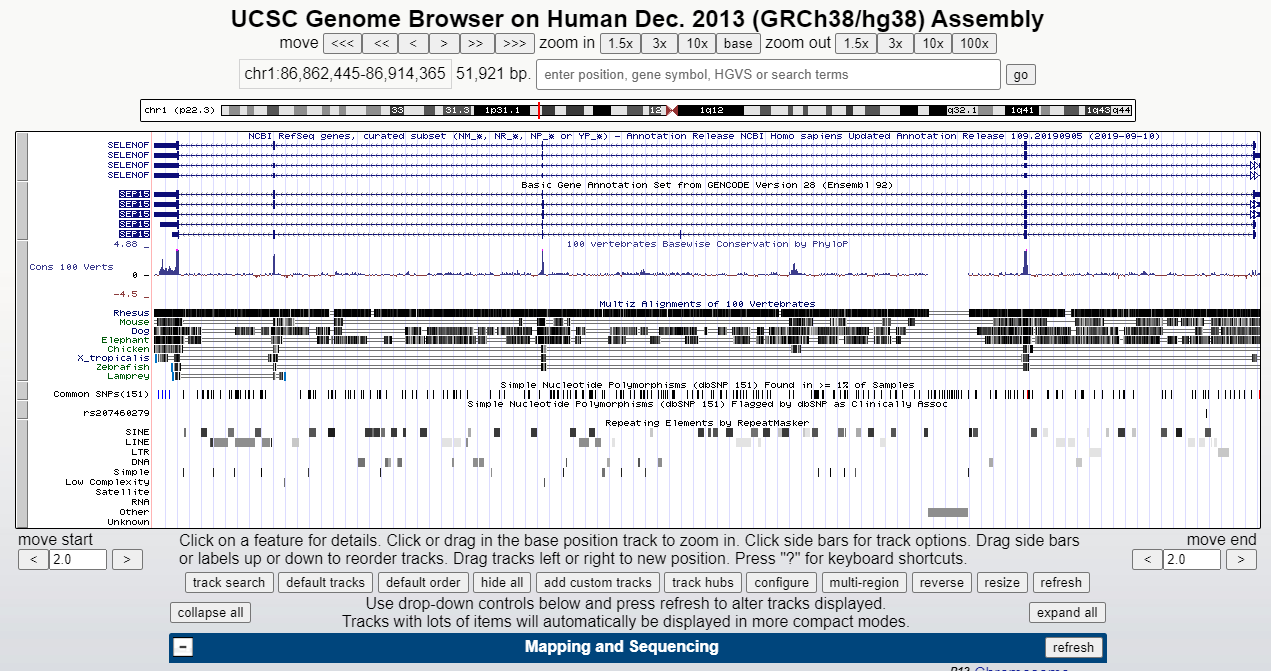
\includegraphics[width=\textwidth]{../bio/hw1/gene_common.png}

  \subsection{Отобрать в табличном виде и сохранить в текстовый файл все изоформы генов, попавших в заданный участок}
  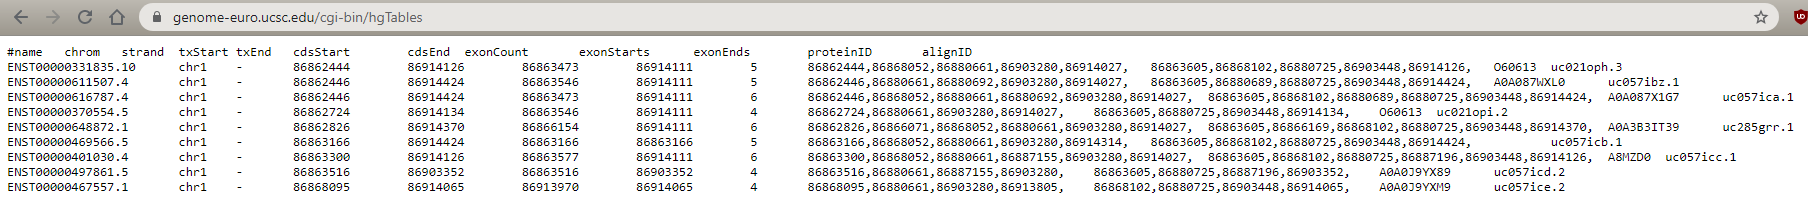
\includegraphics[width=\textwidth]{../bio/hw1/textfile.png}
  он получился какойто слишком маленький (всего 2 килобайта)
  \textattachfile{../bio/hw1/table.txt}{\textcolor{blue}{файл вложенный в pdf (может у когото сработает)}}

  \subsection{Отобрать координаты только экзонов и только интронов для заданного участка}
  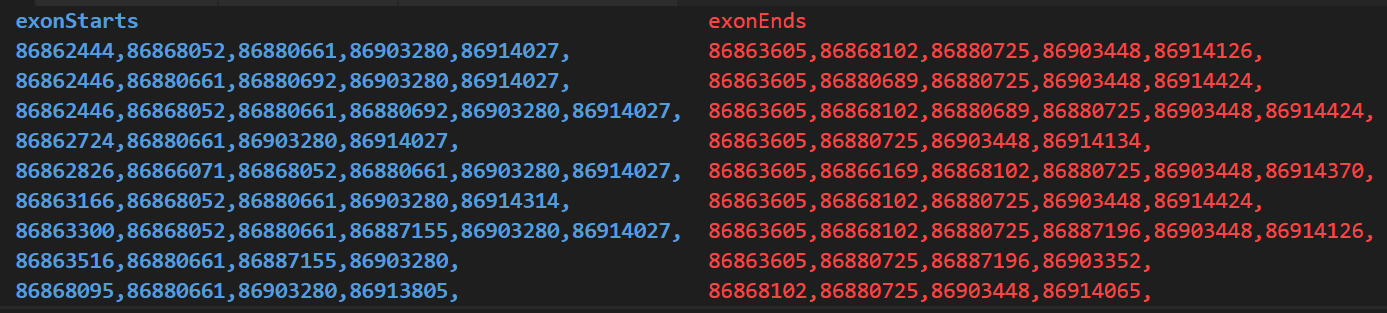
\includegraphics[width=\textwidth]{../bio/hw1/exon.png}
  тут в табличке из второго пункта прописаны координаты экзонов, но они относительно начала хромосомы \\
  мы можем вычесть координату начала гена и получить внутренние координаты (хотя зачем) \\
  получится чтото типа \texttt{0-1161 5608-5658 18217-18281 40836-41004 51583-51682}


  \subsection{Ответить письменно, в какие участки гена попадают clinically relevant SNPs}
  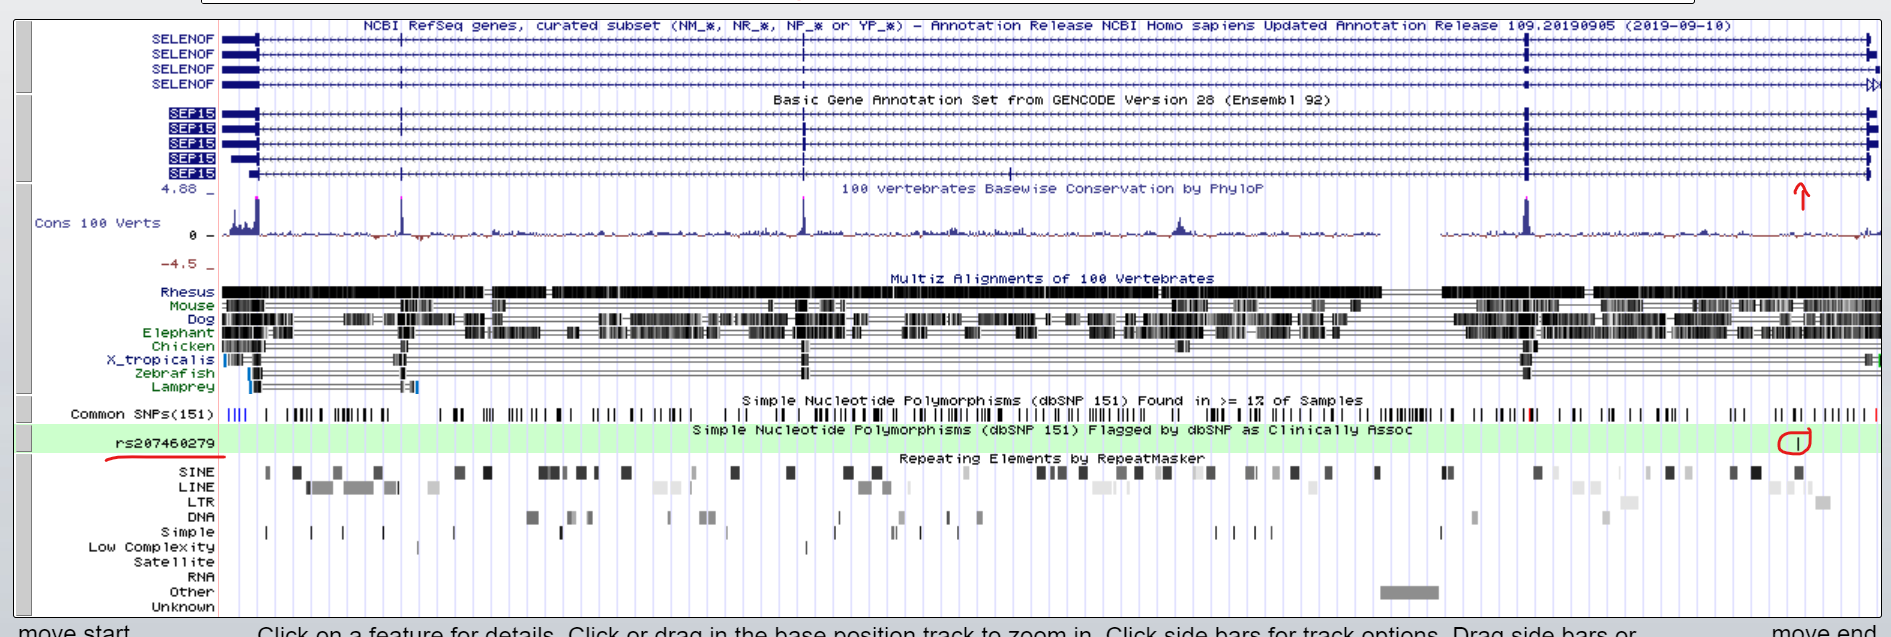
\includegraphics[width=\textwidth]{../bio/hw1/snip.png}
  clinically relevant snip у нас тут только один (rs207460279) попадает на интрон \\
  также если они попадают в экзон то они отмечаются красным

  \subsection{Ответить письменно, в какие участки гена попадают транспозоны}
  
\includegraphics[width=\textwidth]{../bio/hw1/copy.png}
  транспозоны не попадают на экзоны (даже если мы сделаем зум и посмотрим внимательно) \\
  тоесть получилось что они у нас все транспозоны лежат в интронах

\end{document}
